\cotefile{156-7}
\scanpage{66}
\mspage{65}

\deleted{On a les \unsure{co} constructions \unsure{de|d'un} $\unsure{L|\mathcal{L}}$ muni de $\parallel$, d'un $\Sigma_L^\circ$, ens des parties de $L$ ``fermées''. Considérons les applications canoniques}

% The opening paragraph and the whole following diagram are cancelled by oblique strokes.
\diagram{\begin{tikzcd}[ampersand replacement=\&, column sep=huge, execute at end picture={\draw ([xshift=-3mm]current bounding box.south west)--([xshift=3mm]current bounding box.north east);}]
\deleted{\Sigma_M^\circ}
  \arrow[r, shift left=1.5ex, "\deleted{A\mapsto A\cap L}"]
\& \deleted{\Sigma_L\overset{\mathrm{def}}{=}\unsure{\mathscr{P}|\mathcal{P}}(L)}
  \arrow[l, shift left=1.5ex, "\deleted{A_S=\{X\in M\mid\operatorname{omb}(X)\subset S\}\mathrel{\leftarrow\!\vert} S}"]
\end{tikzcd}}

Cette \unsure{relation} entre supports dans $\unsure{\mathcal{F}|\mathscr{F}}$, et supports dans $M$, \unsure{marcherait} en remplaçant $M$ par un \unsure{sous-ensemble} $\Lambda\subset\mathcal{F}$, soumis à la seule condition que voici :

\noindent\begin{tabular}{|p{0.93\linewidth}}
$\underline{\mathrm{Disj}}_\Lambda$ : Soit $F\in\mathcal{F}$, $\operatorname{omb}_\Lambda(F)=\{X\in\Lambda\mid X\ll F\}$.
Alors pour tout $G\in\mathcal{F}$, on a
\[
F\parallel G\quad\Longleftrightarrow\quad\forall X\in\operatorname{omb}_\Lambda(F),\quad X\parallel G
\]
\end{tabular}

Posant, pour $A\subset\mathcal{F}$
\[
\operatorname{omb}_\Lambda(A)\overset{\mathrm{def}}{=}\bigcup_{F\in A}\operatorname{omb}_\Lambda(F)\subset\Lambda,
\]
on voit bien que pour tte partie $A\in\mathcal{F}$, on a
\[
\operatorname{cosupp}_{\mathcal{F}}A=\operatorname{cosupp}_{\mathcal{F}}\operatorname{omb}_\Lambda A.
\]

De plus, si $A$ est fermé dans $\deleted{\unsure{F}}\mathcal{F}$ pour $\ll$, alors on voit aussitôt que
\[
\operatorname{omb}_\Lambda(A)=\Lambda\cap A\qquad(A\text{ fermé ds }\mathcal{F},\ll)
\]
(en général on a seulement $\supset$). Donc on conclut
\[
\operatorname{cosupp}_{\mathcal{F}}(A)=\operatorname{cosupp}_{\mathcal{F}}A\cap\Lambda
\qquad\begin{aligned}&\text{si }A\text{ fermé}\\&\text{dans }\mathcal{F}\text{ pour }\ll\end{aligned}
\]

Ceci implique, en \unsure{reprenant} les supports
\[
\deleted{\unsure{\Sigma_A|A}}\operatorname{supp}_{\mathcal{F}}(A)=\deleted{\unsure{\mathrm{co}}}\operatorname{supp}_{\mathcal{F}}(A\cap\Lambda)
\qquad\begin{aligned}&\text{si }A\text{ fermé}\\&\text{dans }\mathcal{F}\text{ pour }\ll\end{aligned}
\]
et sans hyp. sur $A$
\[
\operatorname{supp}_{\mathcal{F}}(A)=\operatorname{supp}_{\mathcal{F}}(\operatorname{omb}_\Lambda(A))
\]

\scanpage{67}
\mspage{66}

On trouve ainsi une correspondance biunivoque entre les ens de $\unsure{\mathcal{F}|\mathscr{F}}$-supports et de $\Lambda$-supports
\diagram{\begin{tikzcd}[ampersand replacement=\&, column sep=large, row sep=small]
\Sigma_{\mathcal{F}}^\circ \arrow[r, shift left=1.2ex] \& \Sigma_\Lambda^\circ \arrow[l, shift left=1.2ex] \\
A \arrow[r, mapsto] \& A\cap\Lambda=\operatorname{omb}_\Lambda(A) \\
\operatorname{supp}_{\mathcal{F}}\unsure{S|\sigma} \arrow[d, equal] \& S \arrow[l, mapsto] \\
\{F\in\mathcal{F}\mid\operatorname{omb}_\Lambda(F)\subset S\} \&
\end{tikzcd}}
respectant les relations d'ordre (inclusion) et le passage au complémentaire, que je vais noter $\unsure{\mathbb{C}|\complement}_{\mathcal{F}},\mathbb{C}_\Lambda$.

On a envie, pour ``comprendre les supports'', de prendre $\Lambda$ aussi petit que possible. Le choix $\unsure{L|\mathcal{L}}$ s'impose, mais cela demande que l'axiome $\mathrm{AtL2}$ soit satisfait --- ce n'est pas \unsure{évident}. Ainsi, on trouve (changeant des notations, en laissant tomber les exposants des $\Sigma$ \dots)
\[
\Sigma_{\mathcal{F}}\simeq\Sigma_M\simeq\Sigma_L
\]
% margin note written slanted
\margin{\uline{NB} La notion de support ne \unsure{dépend} \unsure{pas} de $\mathcal{F}$ \unsure{que|ou} \unsure{par} \unsure{l'inclusion|l'ensemble} des \unsure{Anatos|Aratos} \unsure{spéci.} Dans le \unsure{cas} $\mathrm{AtL2}$, il ne \unsure{dépend} \unsure{donc} que de $L$, \unsure{et} de la relation $\parallel_L$.}
(sous-entendu à chaque fois : la notion d'ens. ordonné des supports, définie en termes de $\parallel_{\mathcal{F}}$ resp $\parallel_M$ resp $\parallel_L$).

Un cas particulièrement \uline{agréable} est celui où ``$x\parallel_L y$'' est la relation tautologique : $x\ne y$ (p.ex cas $\unsure{\gamma}$ d'un \unsure{Anatos|Aratos} quasi-ensembliste)

\scanpage{68}
\mspage{67}

on trouve
\[
\Sigma_{\unsure{L|\mathcal{L}}}=\unsure{\mathscr{P}|\mathcal{P}}(L),
\]
l'opération $C_L$ étant simplement le passage au complémentaire. Donc dans ce cas, le support d'une partie $A$ de $\unsure{\mathcal{F}|\mathscr{F}}$ (ou de $M$, quand on part des \unsure{Anatos|Aratos}) ; identifié à une partie de $L$, n'est autre que $\operatorname{omb}_L(A)=\operatorname{omb}(A)$. Donc dans ce cas, la définition revient simplement à poser
\[
\begin{aligned}
\operatorname{supp}A&=\operatorname{omb}(A)\overset{\mathrm{def}}{=}\bigcup_{F\in A}\operatorname{omb}(F)\\
\operatorname{cosupp}A&=\unsure{\complement|C}_L\operatorname{supp}A
\qquad\begin{gathered}\text{(complémentaire}\\\text{ordinaire)}\end{gathered}
\end{aligned}
\]

Ceci tient au fait que la relation cruciale de disjonction devient simplement
\diagram{\begin{tikzcd}[ampersand replacement=\&, column sep=small, row sep=large]
F\parallel G\quad\Longleftrightarrow\quad\operatorname{omb}F\cap\operatorname{omb}G={} \& \varnothing \arrow[d, bend right=15] \& {,} \\
\text{relation de disjonction} \& \text{ensembliste} \& \text{sur les}
\end{tikzcd}}
omb (\unsure{rebaptisés} supports pour la circonstance). Dans ce cas, les propriétés p.63,64 se \unsure{résolvent}, on a
\[
\left\{\begin{aligned}
A\subset B&\quad\Longleftrightarrow\quad A\cap\underset{\substack{\uparrow\\\text{``compl.''}}}{\unsure{\mathbb{C}|\complement}}(B)=\varnothing_\Sigma\\
A\cap\bigvee_i B_i&=\bigvee_i A\cap B_i\qquad\text{dans }\Sigma\quad-
\end{aligned}\right.
\]

\scanpage{69}
\mspage{68}
% A long oblique cancellation crosses the body of this draft, reaching the final paragraph.

\deleted{Ceci peut se généraliser ainsi. Soit}
\[
\deleted{P\subset\unsure{L|\mathcal{L}}}
\]
\margin{$P$ comme ``points''}
\deleted{une partie de $L$ (ou simplement de $\unsure{\mathcal{F}|\mathscr{F}}$ --- mais pratiquement ce sera tjrs $\subset L$ je présume) telle que}

\deleted{a) si $x,y\in P$, $x\ne y\Rightarrow x\parallel y$ (donc sur $P$, $x\parallel y$ équivaut à $x\ne y$)}

\deleted{b) si $F,G\in\mathcal{F}$ (resp. $M\unsure{\}}$, si on part de $M$) \unsure{et}}

\deleted{\unsure{alors} \unsure{et si} $\forall x\in\operatorname{omb}_{\unsure{\Lambda|P}}(F),\ y\in\operatorname{omb}_{\unsure{\Lambda|P}}(G)$, on a}

\[
\deleted{\unsure{F\parallel G}}
\]
\deleted{On a $F\parallel G$ si (\unsure{et s.s.|et ss.}) $\nexists x\in P$, $\unsure{\operatorname{supp}x\subset\operatorname{supp}F}$}
\inserted{\deleted{avec $\operatorname{supp}x\subset\operatorname{supp}A\cap\operatorname{supp}B$}}

\deleted{\unsure{si} $x\parallel y$, alors $F\parallel G$}

\deleted{(C'est la condition $\unsure{\mathrm{AtP2}|\mathrm{At}\Lambda2}$, \unsure{i.e.|ou} $\mathrm{At}\Lambda2$ dans le cas $\Lambda=P$ --- condition qui implique $\mathrm{AtL2}$.)}

% margin note written slanted; its arrow points to the paragraph beginning Alors.
\margin{Un peu bref ! $\downarrow$}
\deleted{Alors l'ens ordonné des supports s'identifie à}
\[
\deleted{\Sigma_P\simeq\unsure{\mathscr{P}|\mathcal{P}}(P),\quad\text{donc}}
\]
\diagram{\begin{tikzcd}[ampersand replacement=\&, column sep=large, execute at end picture={\draw ([xshift=-1mm]current bounding box.north west)--([xshift=1mm]current bounding box.south east);}]
\deleted{\unsure{s}}\quad\deleted{A} \arrow[r, mapsto] \& \deleted{\{x\in P\mid\operatorname{supp}x\subset A\}} \\
\deleted{\Sigma_{\deleted{\unsure{\mathcal{F}}}\unsure{F|\mathcal{F}}\text{ (ou }M\text{, ou }L\text{)}}} \arrow[r, phantom, "\deleted{\simeq}"] \& \deleted{\mathscr{P}(P)}
\end{tikzcd}}
\deleted{iso d'ens. ordonnés, compatible à l'application $C$ (``complémentaire''). Donc dans ce cas encore, les perplexités \unsure{s'évanouissent}. Dans ce cas, il y a lieu de définir le support comme}
\[
\deleted{\operatorname{supp}A=\operatorname{omb}_\Lambda A=\bigcup_{F\in A}\operatorname{omb}_\Lambda(F).}
\]

\deleted{Notons que l'isom. d'ens. ordonnés avec \unsure{opération} ``passage au complémentaire''}
\[
\deleted{\Sigma\simeq\mathscr{P}(P)}
\]

\scanpage{70}
\mspage{69}

(25 \unsure{juin|Juin})

En dehors du cas quasi-ensembliste, je suspecte que la notion de support, telle qu'elle est présentée ici, est \unsure{cornée|cornue|connerie} --- qu'il ne faudrait parler de support d'une partie $A$ de $M$, disons, que quand les $X\in A$ sont mutuellement compatibles, ou du moins, si deux à deux ils admettent des subdivisions mutuellement compatibles. Voici un exemple typique.

\uline{Exemple} Stratos associé à un \deleted{segment}\inserted{ens.} ordonné $I$ (p.ex. un ``\uline{segment} ordonné'').
\[
M=M_0\amalg M_1
\]
$M_0$ (0-strates) $=\deleted{\unsure{I}}$\inserted{ens des parties \unsure{uniponctuelles} de $I$} $(=\operatorname{Drap}_0(I))$

% The following initial definition and its accompanying notes are cancelled together.
\deleted{$M_1$ (1-strates) $=\operatorname{Drap}_1(I)\simeq\{(a,b)\in I\times I\mid a<b\}$}
\inserted{\deleted{parties de $I$ de la forme $X_{ab}=\{x\mid a\leq x\leq b\}$ où $a<b$. Alors $a,b$ \unsure{uniquement déterminés}}}
\margin{\deleted{Pour $X\in M_1$ \unsure{défini} par $(a,b)$, on \unsure{écrira} $\partial X=\{a,b\}\subset M_0$. On}}
\[
\deleted{X\leq Y\quad\text{ssi}\quad X\subset Y\quad\text{donc}\quad
\left(\begin{gathered}X<Y\quad\text{ssi}\quad X\in M_1,\ Y\in M_1\\X\in\partial Y\end{gathered}\right)}
\]
\[
\deleted{X\ll Y\quad\text{ssi}\quad\{}
\]
% The opening brace above is abandoned on the manuscript; no condition is written after it.

$M_1$ (1-strates) $=$ ens des sous-segments de $I$, i.e. parties \inserted{$X$} de la forme $I_{a\leq\cdot\leq b}$, où $a<b$. (NB $a,b$ sont uniquement déterminés : origine et extrémité de $X$. On pose $\partial X=\{a,b\}$.

\[
X\leq Y\quad\Longleftrightarrow\quad
\left\{\begin{aligned}&X=Y\text{ ou}\\&X\in M_0,\ Y\in M_1,\quad X\in\partial\deleted{\unsure{X}}Y\end{aligned}\right.
\]
\margin{(dans ce cas, on écrit $X\triangleleft Y$\deleted{\unsure{ou} \unsure{l'inclusion} \unsure{d'incidence} $X\unsure{\triangleleft}Y$})}
\[
X\ll Y\quad\Longleftrightarrow\quad X\subset Y
\]
% The upward stroke at the replacement may be an insertion pointer rather than a quantifier.
\margin{($X\overset{\circ}{\ll}Y$ signifie $X\unsure{\ne}Y$ ou $\deleted{\unsure{X\triangleleft Y}}\inserted{\unsure{X\triangleleft Y|\nexists X\triangleleft Y}}$)}
\inserted{On est dans un des trois cas mutuellement exclusifs}
\[
X\unsure{\bowtie|\gtrless}Y\quad\Longleftrightarrow\quad
\left\{\begin{aligned}
&\text{\textcircled{a}}\ X=Y\quad\deleted{\text{ou}}\quad
\text{\textcircled{b}}\ X\in\partial Y\text{ ou }Y\in\partial X,\quad\deleted{\text{ou}}\\
&\qquad\text{(cas où }Y\text{ resp. }X\text{ est dans }M_1\text{).}\\
&\text{\textcircled{c}}\ \partial X\cup\partial Y,\ \text{tot. ordonné}\\
&\deleted{\unsure{X\cap Y=\varnothing|X\cup Y=\varnothing}}\\
&\deleted{\unsure{\partial X\cap Y|\partial X\cap\partial Y}}\\
&\text{et }X\cap Y\text{ est vide, ou réduit }\deleted{\unsure{X}}\inserted{\text{à}}\text{ un point, }\text{\uline{d'où}}
\end{aligned}\right.
\]
on est dans un des cas : $\alpha)$ $\exists a\leq b<c\leq d$ avec $X=[a,b]$, $Y=[c,d]$ \inserted{ou l'inverse} ou $\beta)$ $\exists a<b<c$ avec $X=[a,b]$, $Y=[\unsure{b},\unsure{c}]$ ou l'inverse.

\figure{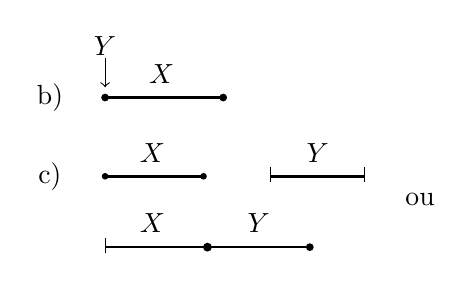
\begin{tikzpicture}[x=1cm,y=1cm]
\node at (-0.7,1.9) {b)};
\draw[line width=0.9pt] (0,1.9)--(1.5,1.9);
\fill (0,1.9) circle (1.4pt);
\fill (1.5,1.9) circle (1.4pt);
\node at (0.72,2.2) {$X$};
\node at (0,2.55) {$Y$};
\draw[->] (0,2.4)--(0,2.03);
\node at (-0.7,0.9) {c)};
\draw[line width=0.9pt] (0,0.9)--(1.25,0.9);
\fill (0,0.9) circle (1.2pt);
\fill (1.25,0.9) circle (1.2pt);
\node at (0.6,1.2) {$X$};
\draw[line width=0.9pt] (2.1,0.9)--(3.3,0.9);
\draw (2.1,0.83)--(2.1,1.02) (3.3,0.83)--(3.3,1.02);
\node at (2.7,1.2) {$Y$};
\node at (4,0.6) {ou};
\draw[line width=0.9pt] (0,0)--(2.6,0);
\draw (0,-0.08)--(0,0.12);
\fill (1.3,0) circle (1.6pt);
\fill (2.6,0) circle (1.4pt);
\node at (0.6,0.3) {$X$};
\node at (1.95,0.3) {$Y$};
\end{tikzpicture}}

\uline{NB}. Tous les axiomes sont satisfaits, à l'exception de $\mathrm{AtL1}$ (\unsure{divisibilité}), satisfait \unsure{ssi|ss} les intervalles $]a,b[$ sont $\ne\varnothing$ $(a<b)$.

\scanpage{71}
\mspage{70}

\uline{NB} Les strates sont combinatoirement finies --- celles de $\unsure{L|\mathcal{L}}=M_0$ sont de dim $0$, celles de $M_1$ de dim $1$. Si $X\in M_0$, $\deleted{\unsure{\widetilde{X}}}\operatorname{card}\widetilde{X}=0$, si $X\in M_1$, $\operatorname{card}\widetilde{X}=3$. On prend pour $\unsure{\mathcal{F}|\mathscr{F}}$ les figures \uline{finies}, i.e. les parties finies $F$ de $M$, \deleted{telles que} fermées pour $\leq$ (i.e. contenant, avec \unsure{tte|tt} $X\in M_1$, ses deux extrémités) et telles que $X,Y\in F\Rightarrow X\unsure{\bowtie|\gtrless}Y$.

\deleted{(\inserted{Comme} \unsure{c'est} ce que dans CF III j'ai appelé ``parties}

\figure{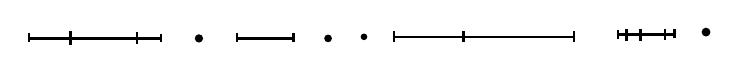
\begin{tikzpicture}[x=0.8cm,y=1cm,line width=0.85pt]
\draw (0,0)--(2.1,0);
\draw (0,-0.05)--(0,0.07) (0.66,-0.08)--(0.66,0.09) (1.72,-0.07)--(1.72,0.08) (2.1,-0.04)--(2.1,0.06);
\fill (2.7,0) circle (1.5pt);
\draw (3.3,0)--(4.2,0);
\draw (3.3,-0.05)--(3.3,0.07) (4.2,-0.05)--(4.2,0.07);
\fill (4.75,0) circle (1.4pt);
\fill (5.32,0.02) circle (1.2pt);
\draw (5.8,0.02)--(8.65,0.02);
\draw (5.8,-0.04)--(5.8,0.09) (6.9,-0.04)--(6.9,0.09) (8.65,-0.04)--(8.65,0.09);
\draw (9.35,0.05)--(10.25,0.05);
\draw (9.35,-0.01)--(9.35,0.11) (9.49,-0.03)--(9.49,0.12) (9.71,-0.03)--(9.71,0.12) (10.1,-0.02)--(10.1,0.12) (10.25,0)--(10.25,0.12);
\fill (10.75,0.08) circle (1.6pt);
\end{tikzpicture}}

Dans CF III, j'ai pris la peine \unsure{essentiellement|éventuellement} de définir le support d'un tel objet comme partie de $I$ (appelée \deleted{\unsure{tout}} ``modérée \unsure{fermée}'', alors que j'aurais dû dire ``modérée'' tout court, et appeler \uline{constructibles} les parties que j'y appelle ``modérées''). Cela donne lieu à un formalisme raisonnable dans le cas \unsure{present|présent|provenant} d'un ens \inserted{fini} de figures ayant la propriété spécifiée au début. Dans le cas d'un ensemble infini, c'est OK si $I$ est un \uline{tronçon} ordonné (loc. cit. p.8) et encore --- toujours est-il que l'on trouve une notion de \uline{parties constructibles} de $I$, de complémentaire d'une telle partie, \deleted{et pour} une notion de compatibilité de parties constructibles, et un bon formalisme des $\bigcup_i,\ \bigcap_i,\ \unsure{\complement|C}$ pour des parties \unsure{constr.|constr} \inserted{$X_\alpha$} deux à deux \deleted{disjointes} compatibles (i.e. telles que la réunion des $\partial X_\alpha$ soit tot.\textsuperscript{t} ordonnée).

\scanpage{72}
\mspage{71}

Je pense qu'on \unsure{arrive|aura} à un tel formalisme sans hyp. sur $I$ (genre ``tronçon ordonné'') à condition de tenir compte de la possibilité qu'il y ait des $1$-strates
\[
X=[a,b]\quad(a<b)
\]
réduites à $\{a,b\}$ (quand $]a,b[=\varnothing$). Dans ce cas, il serait déraisonnable de définir $\operatorname{supp}X=[a,b]$ \unsure{ce qui donne} $=\deleted{\unsure{\{a,b\}}}\operatorname{supp}\partial X$. Mais on doit pouvoir définir une notion de support, \unsure{p. associé} à une partie tot. ordonnée quelconque $\Delta$ de $I$ (\unsure{éventuellement}, $\Delta=\bigcup_\alpha\partial X_\alpha$)
\[
a_1<a_2\ \cdots\ <a_n
\]
comme étant \deleted{\unsure{tous les}} les éléments de l'algèbre de Boole sur l'ens des ``points''
\[
\{a_1\},[a_1,a_2],\{a_2\},[a_2,a_3],\ldots,\{a_n\}
\]

\deleted{Toute famille}\inserted{Pour} $\unsure{\mathscr{X}|\mathcal{X}}\subset M$, $\mathscr{X}=\{X_\alpha\}$, \uline{subordonnée} à $\Delta$ i.e. telle que $\partial X_\alpha\subset\Delta\quad\forall\alpha$, on définit $\operatorname{supp}\mathscr{X}$ comme partie de cet ens (partie fermée, en fait, qui est un ens ordonné de façon évidente\unsure{\}|)}, \unsure{sous|suivant} l'inclusion des \inserted{\unsure{vraies}} parties de $I$), et on définit de même le support d'une différence virtuelle $X\setminus Y$ pour $Y\ll X$, ou $F\setminus G$ pour $F\unsure{\ll|\leq}G$, $F,G$ figures dans la \deleted{\illegible{1}} partie $\leq$-fermée de $\unsure{\mathcal{F}|\mathscr{F}}$ engendrée par $\mathscr{X}$.

Mais ça signifie finalement que pour tte figure dans \unsure{une|un} chaîne, i.e.
\figure{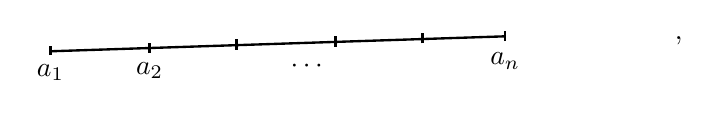
\begin{tikzpicture}[x=1.05cm,y=1cm,line width=0.85pt]
\draw (0,0)--(5.5,0.19);
\draw (0,-0.05)--(0,0.07) (1.2,-0.02)--(1.2,0.11) (2.25,0.02)--(2.25,0.15) (3.45,0.06)--(3.45,0.19) (4.5,0.1)--(4.5,0.23) (5.5,0.13)--(5.5,0.26);
\node[below] at (0,-0.04) {$a_1$};
\node[below] at (1.2,-0.01) {$a_2$};
\node[below] at (3.1,0.02) {$\cdots$};
\node[below] at (5.5,0.11) {$a_n$};
\node at (7.6,0.13) {,};
\end{tikzpicture}}
